\documentclass[a4paper,12pt]{report}

\usepackage[utf8x]{inputenc}
\usepackage[T2A]{fontenc}
\usepackage[english, russian]{babel}
\usepackage[table]{xcolor}

% Опционно, требует  apt-get install scalable-cyrfonts.*
% и удаления одной строчки в cyrtimes.sty
% Сточку не удалять!
% \usepackage{cyrtimes}

% Картнки и tikz
\usepackage{graphicx}
\usepackage{tikz}
\usetikzlibrary{snakes,arrows,shapes}


% Увы, поля придётся уменьшить из-за листингов.
\topmargin -1cm
\oddsidemargin -0.5cm
\evensidemargin -0.5cm
\textwidth 17cm
\textheight 24cm

\sloppy



% Оглавление в PDF
\usepackage[
bookmarks=true,
colorlinks=true, linkcolor=black, anchorcolor=black, citecolor=black, menucolor=black,filecolor=black, urlcolor=black,
unicode=true
]{hyperref}

% Для исходного кода в тексте
% \newcommand{\Code}[1]{\texttt{#1}}

% Некоторая русификация.
% \usepackage{misccorr} % Oh shi^W^W, оно не работает с report.
\usepackage{indentfirst}
\renewcommand{\labelitemi}{\normalfont\bfseries{--}}

% На дворе XXI век, но пакет listings всё ещё не пашет с русскими комментариями!

% Пакет listings для простой вставки исходников
% \usepackage{listings}
% Параметры оформления
% \lstset{
% showspaces=false,
% showtabs=false,
% frame=single,
% tabsize=4,
% basicstyle=\ttfamily,
% identifierstyle=\ttfamily,
% commentstyle=\itshape,
% stringstyle=\ttfamily,
% keywordstyle=\ttfamily,
% breaklines=true
% }
% Русский в комментариях.
% \lstset{escapebegin=\begin{cyr},escapeend=\end{cyr}}

\usepackage{ifthen}
\ifx\requestedLaTeXdate\undefined
\usepackage{array}
\else
\usepackage{array}[=2016-10-06]
\fi
%%
% Packages required by doxygen
\usepackage{fixltx2e}
\usepackage{calc}
\usepackage{doxygen}
\usepackage{graphicx}
\usepackage{makeidx}
\usepackage{multicol}
\usepackage{multirow}
\PassOptionsToPackage{warn}{textcomp}
\usepackage{textcomp}
\usepackage[nointegrals]{wasysym}
\usepackage{ifpdf,ifxetex}

% NLS support packages
\usepackage[T2A]{fontenc}
\usepackage[russian]{babel}

% Font selection
\usepackage[T1]{fontenc}
\usepackage[scaled=.90]{helvet}
\usepackage{courier}
\usepackage{amssymb}
\usepackage{sectsty}
\renewcommand{\familydefault}{\sfdefault}
\allsectionsfont{%
  \fontseries{bc}\selectfont%
  \color{darkgray}%
}
\renewcommand{\DoxyLabelFont}{%
  \fontseries{bc}\selectfont%
  \color{darkgray}%
}
\newcommand{\+}{\discretionary{\mbox{\scriptsize$\hookleftarrow$}}{}{}}

% Arguments of doxygenemoji:
% 1) ':<text>:' form of the emoji, already "LaTeX"-escaped
% 2) file with the name of the emoji without the .png extension
% in case image exist use this otherwise use the ':<text>:' form
\newcommand{\doxygenemoji}[2]{%
  \IfFileExists{./#2.png}{\raisebox{-0.1em}{\includegraphics[height=0.9em]{./#2.png}}}{#1}%
}
% Page & text layout
\usepackage{geometry}
\geometry{%
  a4paper,%
  top=2.5cm,%
  bottom=2.5cm,%
  left=2.5cm,%
  right=2.5cm%
}
\tolerance=750
\hfuzz=15pt
\hbadness=750
\setlength{\emergencystretch}{15pt}
\setlength{\parindent}{0cm}
\newcommand{\doxynormalparskip}{\setlength{\parskip}{3ex plus 2ex minus 2ex}}
\newcommand{\doxytocparskip}{\setlength{\parskip}{1ex plus 0ex minus 0ex}}
\doxynormalparskip
\makeatletter
\renewcommand{\paragraph}{%
  \@startsection{paragraph}{4}{0ex}{-1.0ex}{1.0ex}{%
    \normalfont\normalsize\bfseries\SS@parafont%
  }%
}
\renewcommand{\subparagraph}{%
  \@startsection{subparagraph}{5}{0ex}{-1.0ex}{1.0ex}{%
    \normalfont\normalsize\bfseries\SS@subparafont%
  }%
}
\makeatother

\makeatletter
\newcommand\hrulefilll{\leavevmode\leaders\hrule\hskip 0pt plus 1filll\kern\z@}
\makeatother

% Headers & footers
\usepackage{fancyhdr}

% Indices & bibliography
\usepackage{natbib}
\usepackage[titles]{tocloft}
\setcounter{tocdepth}{3}
\setcounter{secnumdepth}{5}
\makeindex

\usepackage{newunicodechar}
  \newunicodechar{⁻}{${}^{-}$}% Superscript minus
  \newunicodechar{²}{${}^{2}$}% Superscript two
  \newunicodechar{³}{${}^{3}$}% Superscript three

% Custom commands
\newcommand{\clearemptydoublepage}{%
  \newpage{\pagestyle{empty}\cleardoublepage}%
}

\usepackage{caption}
\captionsetup{labelsep=space,justification=centering,font={bf},singlelinecheck=off,skip=4pt,position=top}

\usepackage{etoc}
\etocsettocstyle{\doxytocparskip}{\doxynormalparskip}
\renewcommand{\numberline}[1]{#1~}


\title{Отчёт по лабораторной работе \textnumero 1}
\author{(Ф.~И.~О)}

\begin{document}

\maketitle

\tableofcontents

\addcontentsline{toc}{chapter}{Введение}
\chapter*{Введение}

Два предложения о содержании отчёта. Для нового абзаца в исходном тексте должна быть пустая строка.

Это~-- шаблон отчёта (вот как оформляется длинное тире, перед котрым идёт неразрывный пробел).


Здесь должно быть вербальное задание.

А вот так оформляются списки:
\begin{itemize}
\item элемент списка;
\item последний элемент списка.
\end{itemize}

Нумерованный список выглядит следующим образом.
\begin{enumerate}
\item Первый элемент.
\item Второй элемент.
\end{enumerate}

\chapter{Аналитический раздел}

\chapter{Конструкторский раздел}

\section{Конечный автомат состояний сервера}

Рис.~\ref{fig:fsm} нагенерил самодельный \textit{fsm2dot} из \textit{autogen} и \textit{dot2tex} на пару \textit{dot}. Никто не мешает изменить параметры типа \textit{rankdir} прямо в \textit{fsm2dot}, если он будет лучше смотреться, например, сверху-вниз.

\begin{figure}
\centering
\includegraphics[width=\textwidth]{include/server_def_dot.pdf}
\caption{Состояния сервера}
\label{fig:fsm}
\end{figure}

\section{Синтаксис команд протокола}

\begin{description}
\item[Команда выхода из сеанса]
\input{include/quit_cmd_regexp.tex}
\end{description}

Для грамматики можно использовать вставку из файла и оформление \textbackslash{}begin\{verbatim\} и \textbackslash{}end\{verbatim\} или пакет \textit{listings}\footnote{На дворе XXI век, но пакет \textit{listings} всё ещё не пашет с русскими комментариями без бубна, и лично я его пока не победил.}.

Для примера воспользуемся автоматической вставкой файла описания параметров программы (не забудьте перенести это в технологический раздел) через утилитку \textit{src2tex}.

AutoGen Definitions options;
prog-name     = server;
prog-title    = "SMTP server";
long-opts;
gnu-usage;    /* GNU style preferred to default */

flag = {
    name      = port;           /* Порт, который слушает сервер */
    value     = p;              /* Краткий флаг (-p) */
    arg-type  = number;
    arg-range = 110;
    arg-range = "1024->65000";
    max       = 1;              /* Не более одного раза */
    min       = 1;              /* Обязательный параметр */
    descrip   = "Port to bind";
};

flag = {
    name      = log_dir;        /* Путь до директории с лог-файлами */
    value     = l;              /* Краткий флаг (-l) */
    arg-type  = string;
    max       = 1;              /* Не более одного раза */
    min       = 0;              /* Необязательный параметр */
    descrip   = "Path to the log directory";
};

flag = {
    name      = mail_dir;       /* Путь к директории с локальными письмами */
    value     = d;              /* Краткий флаг (-d) */
    arg-type  = string;
    max       = 1;              /* Не более одного раза */
    min       = 0;              /* Необязательный параметр */
    descrip   = "Path to the maildir directory";
};
% \lstset{language=C}
% \lstinputlisting{../src/checkoptn.def}

\chapter{Технологический раздел}

Нужно отметьть, что символ <<\_>> необходимо оформлять как <<\textbackslash\_>>.

\section{Сборка программы}

Сборка программы описана в файле \textit{Makefile} системы сборки \textit{make}. Рис.~\ref{fig:make} нагенерили самодельные \textit{makesimple} и \textit{makefile2dot}, а также \textit{dot2tex} и \textit{dot}.

Отмечу, что за исключения целей типа \textit{all}, \textit{install}, \textit{clean}, \textit{tests}, все имена целей в файле систем сборки \textit{make} обычно совпадают с именами файлов (такой вот низкоуровневый инструмент). То есть вместо цели \textit{lexer} следует использовать цель \textit{src/lexer.c}.

\section{Основные функции программы}

Весь это раздел сгеренерировал doxygen из части комментированных исходников программы. В файле конфигурации \textbf{doxyggen.cfg} был отключён параметр \textbf{HAVE\_DOT}, поскольку для рисования графов вызовов используется \textit{cflow}.

\hypertarget{main_8c}{}\subsection{Файл main.\+c}
\label{main_8c}\index{main.\+c@{main.\+c}}


Main entry point file.  


\subsubsection*{Структуры данных}
\begin{DoxyCompactItemize}
\item 
struct \hyperlink{structoptions__struct}{options\+\_\+struct}
\begin{DoxyCompactList}\small\item\em Client options struct. \end{DoxyCompactList}\end{DoxyCompactItemize}
\subsubsection*{Определения типов}
\begin{DoxyCompactItemize}
\item 
typedef struct \hyperlink{structoptions__struct}{options\+\_\+struct} \hyperlink{main_8c_a30bf13acdd62b5624d37afb6f89a6e0c}{options\+\_\+t}\hypertarget{main_8c_a30bf13acdd62b5624d37afb6f89a6e0c}{}\label{main_8c_a30bf13acdd62b5624d37afb6f89a6e0c}

\begin{DoxyCompactList}\small\item\em Client options struct. \end{DoxyCompactList}\end{DoxyCompactItemize}
\subsubsection*{Функции}
\begin{DoxyCompactItemize}
\item 
static void {\bfseries close\+\_\+handler} (int signal)\hypertarget{main_8c_adafcb2d413890485316dc00bbd87d2f0}{}\label{main_8c_adafcb2d413890485316dc00bbd87d2f0}

\item 
int \hyperlink{main_8c_a859307c43da5908cb529781d87068c29}{main\+\_\+loop} ()\hypertarget{main_8c_a859307c43da5908cb529781d87068c29}{}\label{main_8c_a859307c43da5908cb529781d87068c29}

\begin{DoxyCompactList}\small\item\em Main client loop func. \end{DoxyCompactList}\item 
\hyperlink{main_8c_a30bf13acdd62b5624d37afb6f89a6e0c}{options\+\_\+t} {\bfseries fill\+\_\+options} ()\hypertarget{main_8c_a0fec7fc1601ea618067b662f02c512cf}{}\label{main_8c_a0fec7fc1601ea618067b662f02c512cf}

\item 
int {\bfseries validate\+\_\+options} (\hyperlink{main_8c_a30bf13acdd62b5624d37afb6f89a6e0c}{options\+\_\+t} options)\hypertarget{main_8c_ada9147964d2cd1be480dd27aae5294c7}{}\label{main_8c_ada9147964d2cd1be480dd27aae5294c7}

\item 
int {\bfseries main} (int argc, char $\ast$$\ast$argv)\hypertarget{main_8c_a3c04138a5bfe5d72780bb7e82a18e627}{}\label{main_8c_a3c04138a5bfe5d72780bb7e82a18e627}

\end{DoxyCompactItemize}
\subsubsection*{Переменные}
\begin{DoxyCompactItemize}
\item 
static volatile int {\bfseries run} = 1\hypertarget{main_8c_a86d4c45d6f679f903dd72e84f4b961c8}{}\label{main_8c_a86d4c45d6f679f903dd72e84f4b961c8}

\item 
static logger\+\_\+t $\ast$ {\bfseries logger}\hypertarget{main_8c_a9575b06719f9ef5b9443b1dc68d38fe4}{}\label{main_8c_a9575b06719f9ef5b9443b1dc68d38fe4}

\item 
static int {\bfseries pipe\+Descrs} \mbox{[}2\mbox{]} = \{ 0, 0 \}\hypertarget{main_8c_affb0b2f4ce744f48e98e0a8aad5b673a}{}\label{main_8c_affb0b2f4ce744f48e98e0a8aad5b673a}

\item 
\hyperlink{main_8c_a30bf13acdd62b5624d37afb6f89a6e0c}{options\+\_\+t} {\bfseries client\+\_\+options}\hypertarget{main_8c_a0b3ee24a66a4de50f4d5714869d1231b}{}\label{main_8c_a0b3ee24a66a4de50f4d5714869d1231b}

\end{DoxyCompactItemize}


\subsubsection{Подробное описание}
Main entry point file. 


\input{include/server_8h.tex}
\input{include/structserver__struct.tex}
\input{include/structserver__client__dict__struct.tex}
\input{include/structserver__client__struct.tex}
\input{include/structmail__struct.tex}

\section{Графы вызова функций}

Поскольку функций много, графы вызовов разбиты на два рисунка. На рис.~\ref{fig:cflow01} показаны основные функции, на рис.~\ref{fig:cflow02}~-- функции обработки команд. Файл \textbf{cflow.ignore} содержит список функций (точнее, шабловнов поиска), использыемых программой \textit{grep} для удаления малоинтересных стандартных функций\footnote{Функции по работе с сокетами, ipc и привилегиями к малоинтересным ни в коем случае не относятся.}.

\begin{figure}
\centering
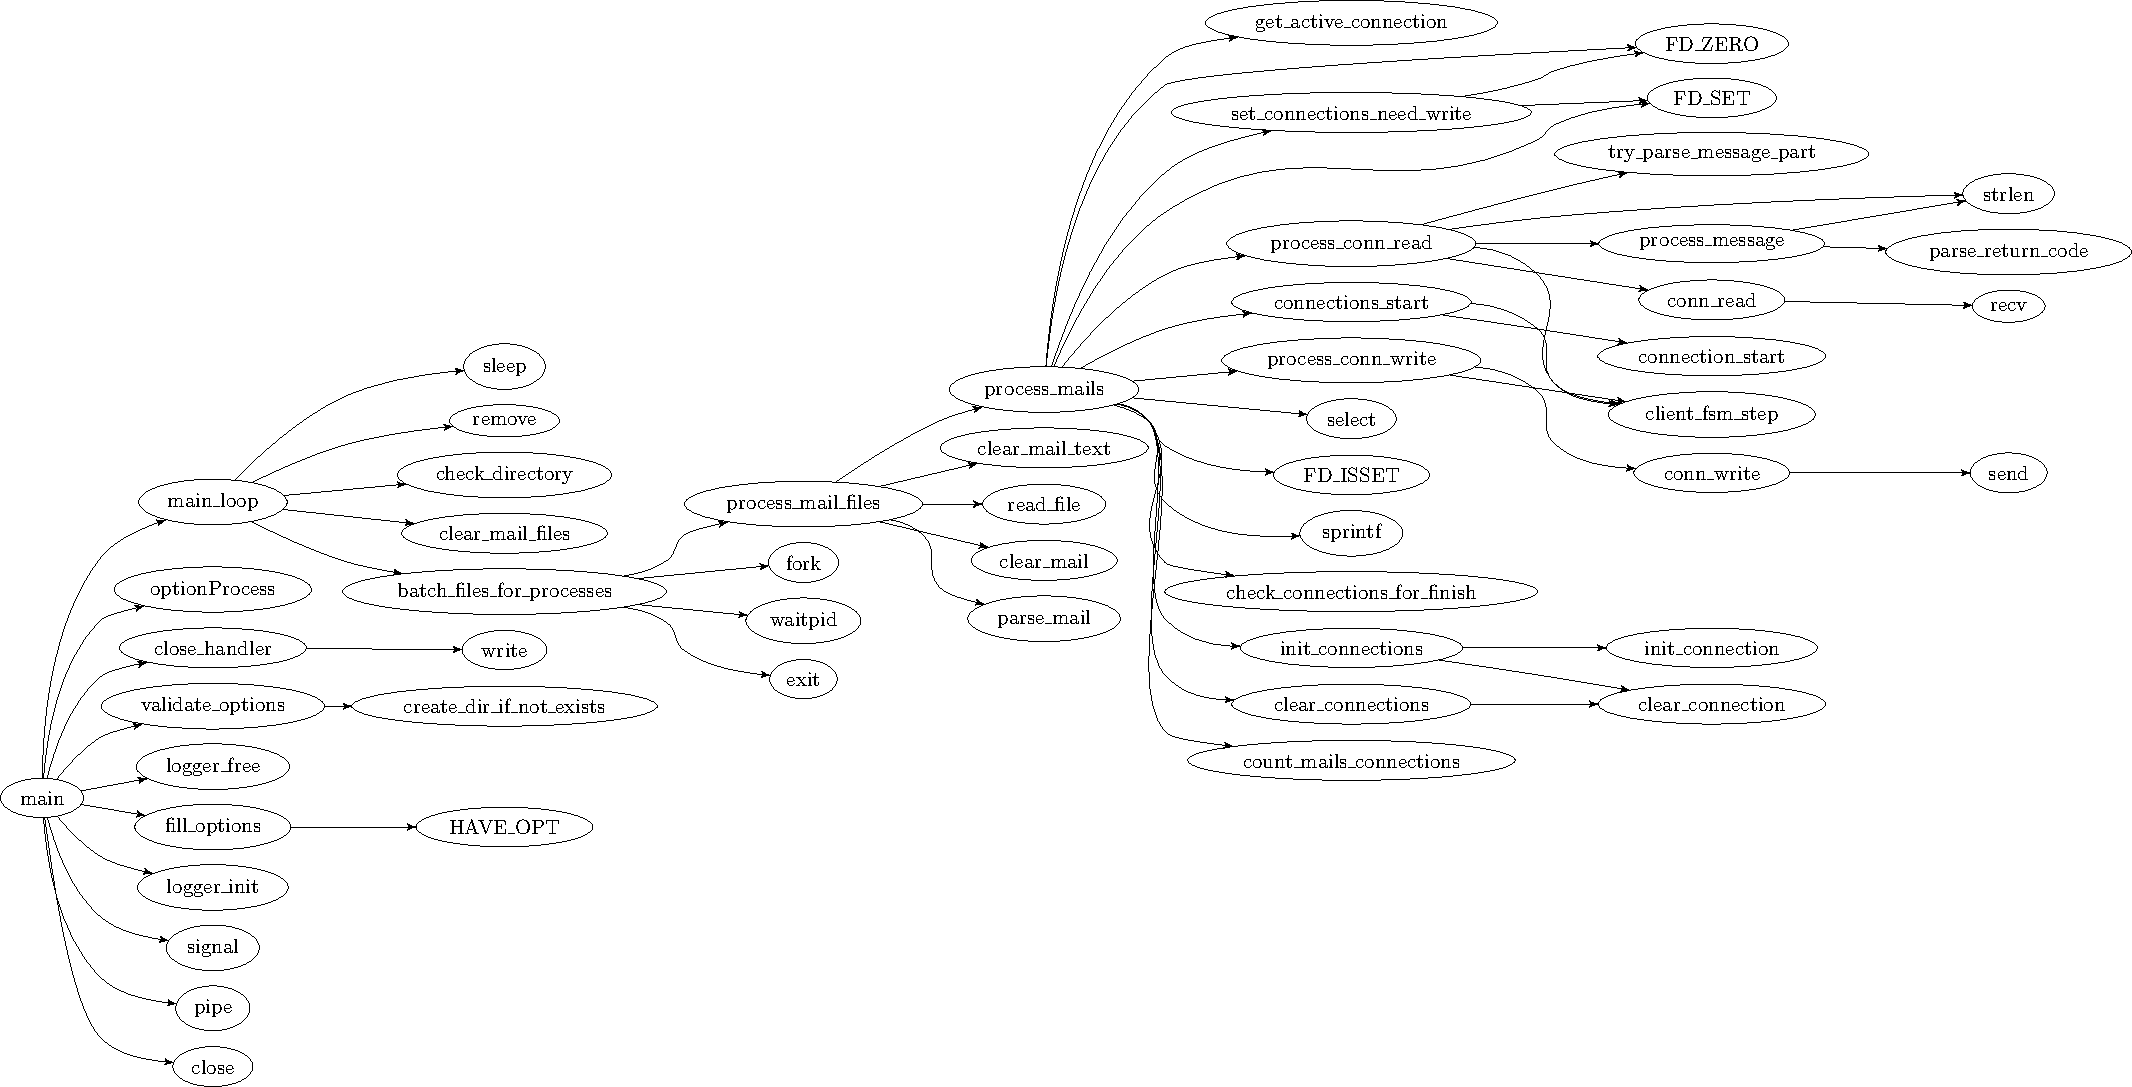
\includegraphics[width=\textwidth]{include/cflow_main_dot.pdf}
\caption{Граф вызовов, основные функции}
\label{fig:cflow01}
\end{figure}

\begin{figure}
\centering
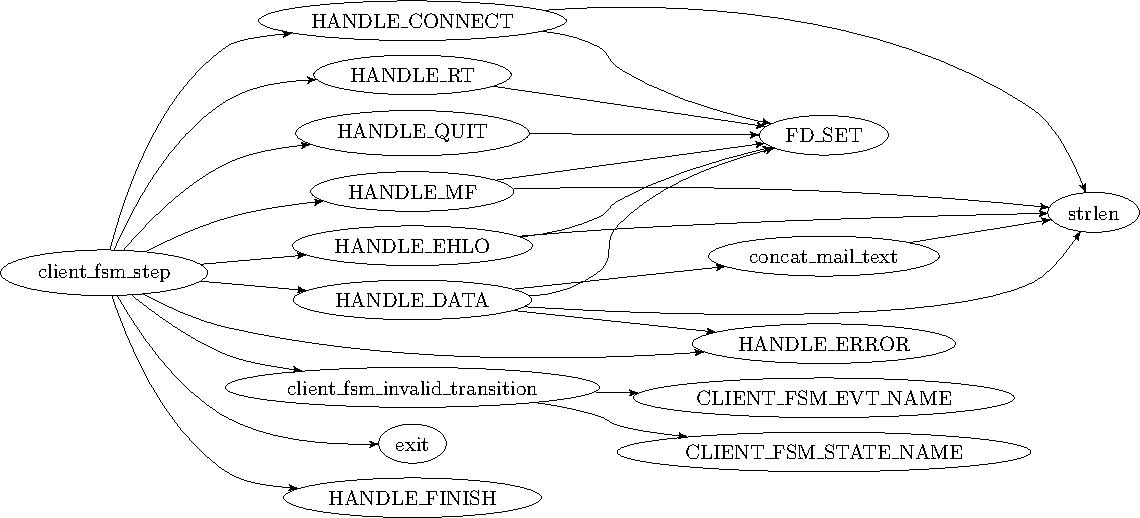
\includegraphics[width=\textwidth]{include/cflow_handlers_dot.pdf}
\caption{Граф вызовов, функции обработки команд}
\label{fig:cflow02}
\end{figure}

Графы созданы с помощью \textit{cflow}, \textit{cflow2dot}, \textit{dot}.

\addcontentsline{toc}{chapter}{Выводы}
\chapter*{Выводы}

Что вы сделали и поняли.


\end{document}
